\documentclass[a4paper,10pt]{article}
\usepackage[french]{babel}
\usepackage[utf8]{inputenc}
\usepackage[top=2cm, bottom=2cm, left=2cm, right=2cm]{geometry}
\usepackage{setspace}
\usepackage[T1]{fontenc}
%\usepackage{listings}
\usepackage{graphicx}
\usepackage{fancyhdr}
\usepackage{color}
\usepackage[table]{xcolor}
\usepackage{listings}
\usepackage{amsmath}
\usepackage{algorithmic}
\usepackage{multicol}
\usepackage{float}
\usepackage{amssymb}
\usepackage{lmodern}
\usepackage[french,boxed,ruled,lined]{algorithm2e}
\definecolor{darkWhite}{rgb}{1.00,1.00,1.00}
\definecolor{light-gray}{gray}{0.95}
\lstset{
framexleftmargin=10mm,
aboveskip=4mm,
belowskip=0mm,
backgroundcolor=\color{light-gray},
breakatwhitespace=false,
captionpos=b,
commentstyle=\color{red},
deletekeywords={...},
escapeinside={\%*}{*)},
extendedchars=true,
keepspaces=true,
language=C,
literate=
{²}{{\textsuperscript{2}}}1
{⁴}{{\textsuperscript{4}}}1
{⁶}{{\textsuperscript{6}}}1
{⁸}{{\textsuperscript{8}}}1
{€}{{\euro{}}}1
{é}{{\'e}}1
{è}{{\`{e}}}1
{ê}{{\^{e}}}1
{ë}{{\¨{e}}}1
{É}{{\'{E}}}1
{Ê}{{\^{E}}}1
{û}{{\^{u}}}1
{ù}{{\`{u}}}1
{â}{{\^{a}}}1
{à}{{\`{a}}}1
{á}{{\'{a}}}1
{ã}{{\~{a}}}1
{Á}{{\'{A}}}1
{Â}{{\^{A}}}1
{Ã}{{\~{A}}}1
{ç}{{\c{c}}}1
{Ç}{{\c{C}}}1
{õ}{{\~{o}}}1
{ó}{{\'{o}}}1
{ô}{{\^{o}}}1
{Õ}{{\~{O}}}1
{Ó}{{\'{O}}}1
{Ô}{{\^{O}}}1
{î}{{\^{i}}}1
{Î}{{\^{I}}}1
{í}{{\'{i}}}1
{Í}{{\~{Í}}}1,
morekeywords={*,...},
numbers=left,
numbersep=10pt,
numberstyle=\tiny\color{black},
rulecolor=\color{black},
showspaces=false,
showtabs=false,
stepnumber=1,
tabsize=4,
title=\lstname,
showstringspaces=false,
basicstyle=\footnotesize\ttfamily,
keywordstyle=\bfseries\color{green!40!black},
identifierstyle=\color{blue},
stringstyle=\color{orange},
}


\begin{document}
\pagestyle{fancy}
\lhead{Projet S6 : Hex Project}
\rhead{\thepage}
\lfoot{}
\cfoot{}
\rfoot{}


\title{Projet S6 : Hex Project }
\author{Ibrahim LMOURID, Houssam BAHHOU, Ayoub LASRI, Eloi Magon De La Villehuchet}


\label{sec:title}
\thispagestyle{empty}



\includegraphics[width=0.4\textwidth]{Logo.png}
\\
\\
\\
\\
\\
\noindent\rule{\textwidth}{1pt}
\begin{flushright}
  \Huge
  \textbf{Rapport de Projet C}

    \vspace{15pt}
  \large 
  \textsl{Hex Project }

\end{flushright}
\noindent\rule{\textwidth}{1pt}

\vspace{\stretch{1}}

\large
\noindent\textbf{Auteurs   : }  \textup{Ibrahim LMOURID \& Houssam BAHHOU \& Ayoub LASRI \& Eloi Magon De La Villehuchet - Equipe $n^{o}$ 9152 } \\
\noindent\textbf{Encadrants :} \textup{ Monsieur Frédéric Herbreteau }
\vspace{\stretch{1}}
\vspace{\stretch{0.5}}

\normalsize
\begin{center}
  Première année, Semestre 6,Filière informatique,ENSEIRB-MATMECA\\
  Date : \today
\end{center}

\vspace{\stretch{1}}


\newpage
\tableofcontents

\newpage
\section{Introduction au jeu de Hex}
\subsection{Contexte et présentation du sujet}
Le jeu de \textbf{\emph{Hex}} a été inventé pour la première fois en 1942 par \textbf{Piet Hein}, un scientifique, mathématicien, écrivain et poète danois. En 1948, \textbf{John Nash}, un mathématicien américain à Princeton a redécouvert le jeu, qui est devenu populaire parmi les étudiants diplômés à Princeton. Ce jeu fait appel à la logique, à l'image des échecs. Son étude fait partie de la théorie des jeux, et d'autres branches mathématiques.\\

Hex est joué avec deux personnes, sur un plateau généralement en forme de losange composé de cellules hexagonales. Les dimensions du plateau de jeu peuvent varier, mais la taille typique est de $11 \times 11$. Deux côtés opposés du plateau sont noirs et les deux autres côtés sont blancs (Figure \ref{fig:board}). Au début de la partie le plateau est vide, les joueurs alternent les tours pour placer leur coup sur n'importe quel espace inoccupé sur le plateau de jeu, en lui assignant leur couleur, dans le but de former une chaîne ininterrompue de pions reliant les deux bords. Un résultat non trivial dont la preuve est liée au théorème de Brouwer affirme qu'il existe toujours un vainqueur (\emph{ie} le match nul n'existe pas au Hex).\\
\begin{figure}[h]
\begin{center}
    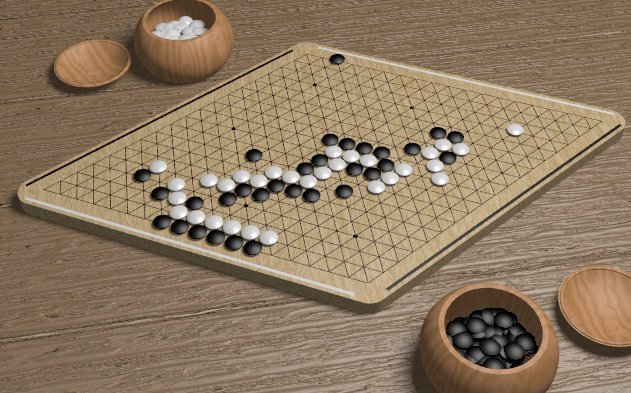
\includegraphics[scale=4.0]{board.jpg}
        \caption{Un exemple du plateau du jeu hexadécimale}
    \label{fig:board}
\end{center}
\end{figure}

\textbf{Convention:} Par convention, dans la suite du rapport, le joueur qui joue avec les pions noires est appelé \textbf{BLACK}, celui qui joue avec les pions blanches, \textbf{WHITE}.\\

Une règle supplémentaire, est la règle du gâteau (\textbf{pie rule} en anglais). Si le joueur \textbf{A} commence, il joue son premier coup noir, l'autre joueur \textbf{B} a alors le choix entre jouer à son tour ou intervertir les couleurs. Dans le 2e cas, le joueur qui a commencé devient alors BLACK, et joue alors son premier coup en tant que BLACK, le jeu continuant ensuite normalement. Cela impose de jouer un premier coup ni trop fort (car donnerait un avantage au joueur adverse qui se l'approprierait) ni trop faible (il serait alors laissé par l'adversaire) et réduit l'avantage de commencer. \\
\subsection{Problématique}
L'objectif du projet était alors d'implémenter une simulation du jeu \emph{Hex} en \texttt{langage C}.\\
Pour ce faire, il a fallu subdiviser le travail de la manière suivante:
\begin{itemize}
    \item L'implémentation du plateau 
    \item La création d'un ensemble de joueurs (clients)
    \item L'implémentation d'un serveur organisant le jeu entre deux clients
\end{itemize}
Le but sous-jacent du projet était de se familiariser avec la manipulation des bibliothèques dynamiques, et d'appliquer les connaissances acquises en théorie des graphes et en programmation impérative. 

\section{Cadre du travail}
\subsection{Outils de travail}
Pour pouvoir partager nos avancements nous avons utilisé Git.\\ Ce logiciel nous a permis d’effectuer un travail collaboratif et de conserver chaque version déposée afin d’éviter les mauvais choix et de pouvoir revenir sur nos pas.\\
Ce compte rendu est rédigé en \LaTeX, les fichiers relatifs à son écriture sont présents sur le dépôt.
\subsection{Architecture des fichiers et détails techniques}
Les fichiers dans le dépôt sont organisés de la manière suivante:\\
\begin{center}
    
    \begin{verbatim}
        /              -- la racine du répertoire du projet
        Makefile       -- Makefile global
        README.md      -- fichier qui contient les instructions d’exécution
        /src           -- fichiers sources (.c/h)
        /install       -- Répertoire Install 
        /rapport       -- Rapport du projet (.tex/pdf)
    \end{verbatim}
        
\end{center}

Le fichier \texttt{Makefile} fournit :
\begin{itemize}
    \item \textbf{une règle \texttt{build}} qui compilera l'ensemble du code,
    \item \textbf{une règle \texttt{test}} qui compilera les tests, sans les exécuter
    \item \textbf{une règle \texttt{install}} qui copiera les exécutables (server, exécutables de tests alltests*, et un nombre non spécifié de fichiers .so) à l'intérieur du répertoire désigné, et
    \item \textbf{une règle \texttt{clean}} qui supprimera les fichiers compilés et installés.
\end{itemize}

Le \texttt{Makefile} prends une variable \texttt{GSL\_PATH} qui indique le répertoire où est installée la bibliothèque \texttt{libgsl.so}.
\section{Structures implémentées et choix effectués}
L'objectif de cette section est de décrire l'ensemble des types abstraits de données et structures implémentées, servant de briques de base à la réalisation du sujet.
\subsection{TAD \texttt{graphe\_t}}
Le tablier du jeu est en fait un système formé de plusieurs cases connectées pouvant se trouver dans plusieurs états au cours du jeu. Par conséquent l'outil le plus propre pour représenter ce jeu est la théorie des graphes.\\
En effet le jeu de \emph{Hex} fait partie des jeux à objectif compétitif sur un graphe, dont les règles et les conditions de victoire sont reliées à un problème d'optimisation, l'idée donc du sujet se trouve dans l'association de chaque plateau du jeu à un graphe grille dont les noeuds représentent les différentes cases du tablier.\\

Le sujet propose de travailler sur trois configurations du plateau avec des tailles variables : Une configuration hexagonale (typique), carrée et triangulaire. Dans notre cas nous avons arrivé à travailler juste sur les deux configurations hexagonale et carrée. \\

Le TAD \texttt{graph\_t}, contient une représentation symbolique du plateau qui nous permet de traiter rapidement et efficacement les différentes opérations du jeu sous forme d’opérations sur les graphes.\\
La structure correspondante à ce TAD a pour champs: 
\begin{itemize}
    \item le nombre de sommets \textbf{\texttt{num\_vertices}} (noté n dans la suite du rapport)
    \item \textbf{La matrice t} qui est une matrice d'adjacence de taille $n\times n$ représentant les arêtes du graphe.
    \item \textbf{La matrice o} qui est une matrice $2\times n$ codant sur chaque ligne les sommets du graphe appartenant au joueur correspondant (donc 0 ou 1)
\end{itemize}

Les deux matrices \textbf{ t et o} sont des matrices creuses, que l'on va définir à l'aide de \texttt{GNU Scientific Library}, une bibliothèque \texttt{C et C++} permettant de faire des calculs numériques, elle fournit aussi des implémentations et des méthodes de matrices denses et creuses, on verra ultérieurement en détail les méthodes associées au \texttt{TAD graph\_t}.
\newpage
\begin{multicols}{2}
\begin{figure}[H]
  \begin{center}
  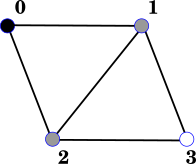
\includegraphics[scale=1.5]{hex4.png}
  \caption{Exemple de graphe hexagonales à 4 sommets}
  \label{fig1}
  \end{center}
\end{figure}
\columnbreak

\begin{center}
$\begin{cases}
    \texttt{num\_vertices}=4 \\
    \texttt{t}=\begin{bmatrix}
        0 & 1 & 1 & 0\\
        1 & 0 & 1 & 1\\
        1 & 1 & 0 & 1\\
        0 & 1 & 1 & 0\\
    \end{bmatrix}\\
    \texttt{o}=\begin{bmatrix}
        1 & 0 & 0 & 0\\
        0 & 0 & 0 & 1\\
    \end{bmatrix}
\end{cases}$
\end{center}
Représentation équivalente du graphe par la structure \texttt{graph\_t}
\end{multicols}
\subsection{TAD \texttt{neighbours}}
Afin d'évaluer la connexité entre les bords du plateau, ou implémenter des méthodes et des opérations sur le graphe, il nécessite d'abord de pouvoir connaître les voisins de chaque sommet dans le graphe. Pour cela on a implémenté le TAD \texttt{neighbours}, dont la structure contient les champs suivants:
\begin{itemize}
    \item \textbf{\texttt{nb}}: tableau alloué dynamiquement.
    \item \textbf{\texttt{size}}: taille de \texttt{nb}
    \item \textbf{\texttt{capacity}}: capacité de \texttt{nb}
\end{itemize}
Ce TAD contient l'implémentation des méthodes qui servent à extraire les voisins de n'importe quel noeud pour les deux configurations implémentées hexagonale et carrée.  

\subsection{TAD \texttt{Path}}
Au cours du jeu les deux joueurs essayent de former des chaînes continues afin de connecter les deux bords du plateau, et donc parmi les possibilités qui existent ils cherchent à construire le bon chemin afin de gagner la partie.\\
Le TAD \texttt{Path} permet donc à l'aide de ses méthodes de stocker le chemin choisit sous forme d'un tableau alloué dynamiquement, la structure \texttt{Path} est la suivante :
\begin{itemize}
    \item \textbf{\texttt{path}}: tableau alloué dynamiquement.
    \item \textbf{\texttt{size}}: taille de \texttt{path}
    \item \textbf{\texttt{capacity}}: capacité de \texttt{path}
\end{itemize}
\subsection{Autres structures}
\begin{enumerate}
    \item Afin de respecter \textbf{la convention} énoncé en Introduction, on a crée un type énuméré \textbf{\texttt{enum color\_t}} qui nous fournit les constantes BLACK=0, WHITE=1, NO\_COLOR=2  correspondant au deux joueurs.
    \item \textbf{\texttt{structure move\_t}}: pour placer un pion dans une position donnée, il faut d'abord donner une représentation symbolique à ce coup, c'est le rôle de la \texttt{structure move\_t} dont les champs correspondent à:
    \begin{itemize}
        \item \textbf{\texttt{m}}: un indice entre 0 et n-1.
        \item \textbf{\texttt{c}}: la couleur du joueur.
    \end{itemize}
    \item \textbf{\texttt{structure player (player-load.h)}:} Chaque client est censé être \textbf{automatique}, et donc il sera manipulé au cours du jeu par le serveur, à l'aide de plusieurs méthodes, par exemple: initialiser la couleur du joueur, ou bien jouer un coup dans son tour... Afin de donner une représentation symbolique à nos clients , on a choisit donc de créer une structure qui contient les pointeurs des fonctions (méthodes) correspondant à chaque joueur(décrites dans l'interface \texttt{player.h}), ces pointeurs de fonctions sont :
    \begin{center}
    
    \begin{lstlisting}
       struct player {
        char const* (*get_player_name)();//avoir le nom du joueur
        struct move_t (*propose_opening)();//proposer le 1er coup
        int (*accept_opening)(const struct move_t);//accepter ou intervertir le 1er coup
        void (*initialize_graph)(struct graph_t*);//initialiser le graphe du joueur
        void (*initialize_color)(enum color_t);//initialiser la couleur du joueur
        struct move_t (*play)(struct move_t);//jouer le coup
        void (*finalize)();//annoncer la fin du jeu
        void * handle;
        };
     \end{lstlisting}
    \end{center}
    \item Dans l'interface \texttt{.c} de chaque joueur (\texttt{player.c , heuristic.c...}) il nous a paru important comme choix de programmation, de regrouper l'ensemble d'informations à propos du joueur (nom, couleur, graphe, nombre de case libre..) sous forme d'une \textbf{\texttt{structure player}} autre que celle décrite avant.  
\end{enumerate}
\section{Méthodes algorithmiques}
\subsection{Plateau du jeu}
L'implémentation d'un plateau du jeu se base sur le TAD \texttt{graph\_t} décrit dans les fichiers \texttt{graph.c, my-graph.c/h }.\\
En fait, les joueurs possèdent des pions à leur couleur qu'ils disposent tour à tour sur une case de leur choix et un par un. Le tablier se remplit ainsi progressivement. La manipulation de ces actions se fait principalement par les fonctions suivantes: 
\begin{itemize}
    \item \textbf{\texttt{graph\_initialize}}: c'est une fonction de plus haut niveau d’abstraction: prend en argument un entier \texttt{size\_t n} et un caractère \texttt{char c} et initialise un tablier vide de nombre de sommets \texttt{n}, et de forme c (hexagonale ou carré) en faisant appel aux fonctions \texttt{initialize\_carre}, \texttt{initialize\_hex} et \texttt{intialize\_o}.
    \newline
    \item \textbf{\texttt{initialize\_o}}: puisqu'on a implémenté que les deux configurations carrée et hexagonale, une implémentation commune de la matrice \texttt{o}  suffit, cette fonction prends la matrice \texttt{o} déjà allouée et l'initialise.
    \newline
    \item \textbf{\texttt{initialize\_carre/hex}}: allouent et renvoient un graphe carré (respectivement Hexagonale) de \texttt{n}  sommets après avoir initialisé ses matrices creuses \texttt{t}  et \texttt{o} .
    \newline
    \item \textbf{\texttt{graph\_display}} Affiche le graphe donné en paramètre selon sa forme, son résultat est ce qu’on peut voir dans la figure
    \newline
    \item \textbf{\texttt{graph\_add\_move}}: cette fonction permet d'ajouter le coup donné en paramètre au graphe correspondant
    \newline
    \item \textbf{\texttt{graph\_free}}: elle sert à libérer tout espace mémoire alloué dans le graphe (matrices creuses t, o et le graphe lui même)
\end{itemize}
\subsection{serveur}
Le serveur est principalement responsable de l’arbitrage, de la coordination des parties, de la préparation et la production de résumés des matches. La première tâche du serveur est d’organiser le mode du jeu à l’aide de la fonction \texttt{parse\_opts}, en utilisant les paramètres données en ligne de commande,
 qu’on peut résumer de la manière suivante:
 \begin{itemize}
     \item  L'option \textbf{\texttt{-m}} permet de spécifier la largeur du plateau de jeu (ex. \textbf{\texttt{-m 11}}). (notation valable pour la suite du rapport)
    \item L'option \textbf{\texttt{-t}} permet de spécifier la forme du plateau de jeu (grille carrée c ou hexagonale h) (ex. \textbf{\texttt{-t h}}).
    \item Les clients sont passés en paramètre dans l'ordre 1er joueur / 2nd joueur
 \end{itemize}
 
Par conséquent, la ligne de commande suivante permet d'exécuter une partie de Hex en chargeant les deux joueurs \texttt{player1.so} et \texttt{player2.so} d'une manière dynamique:
\begin{verbatim}
    ./install/server -m [M] -t [T] ./install/player1.so ./install/player2.so
\end{verbatim}

Ensuite, les deux joueurs chargés sont stocké dans le tableau \texttt{players[2]}  en utilisant
les fonctions \texttt{dlopen, dlsym, dlerror et dlclose}, fournies par la Dynamic Loaded (DL) Libraries. Après, le serveur se charge d’initialiser les différents plateaux de jeu correspondant aux serveur, player1 et player2.\\
Maintenant que tout est prêt, le serveur lance le jeu, le 1er joueur passé en ligne de commande propose le premier coup, puis \textbf{la règle de gâteau} (décrite en introduction) intervient pour permettre au  serveur de déterminer le joueur \textbf{BLACK} et \textbf{WHITE}, et la boucle du jeu continue.\\

Finalement, le serveur arrête le jeu et affiche les résultats de
la partie une fois que la fonction \textbf{\texttt{is\_winning}} lui annonce un gagnant, ou que le plateau est plein. La boucle du jeu correspond au pseudo-algorithme suivant:\\
\begin{algorithm}
\caption{Boucle du jeu}
\begin{algorithmic}
\FOR{ each player p}
    \STATE p$\rightarrow$initialize\_graph(graph)
\ENDFOR    
\STATE move = first\_player$\rightarrow$propose\_opening()
\IF{ second\_player$\rightarrow$accept\_opening(move) // 2nd player plays next}
\STATE first\_player$\rightarrow$initialize\_color(BLACK)
\STATE second\_player$\rightarrow$initialize\_color(WHITE)
\ELSE[// 2nd player refuses and 1st player plays next]
\STATE first\_player$\rightarrow$initialize\_color(WHITE)
\STATE second\_player$\rightarrow$initialize\_color(BLACK)
\ENDIF
\WHILE{true} 
\STATE p = compute\_next\_player()
\STATE move = p$\rightarrow$play(move)
\IF{the board is full}
\STATE break
\ENDIF
\IF{is\_winning()}
\STATE break
\ENDIF
\ENDWHILE
\FOR{each player p}
\STATE p$\rightarrow$finalize()
\ENDFOR
\end{algorithmic}
\end{algorithm}
\newpage
Concernant la fonction \textbf{\texttt{is\_winning}}, son objectif est de vérifier qu'il existe un vainqueur, autrement dit qu'il existe deux cotés opposés reliés, pour cela il faut parcourir la grille en cherchant un chemin connectant ces deux bords. On a choisit donc d'implémenter cette fonction en se basant sur \textbf{un algorithme de recherche en profondeur}.\\

\textbf{L'algorithme} commence au nœud racine (\textit{i.e.\ } \textbf{0} dans le cas d'un joueur BLACK et \textbf{m+1} pour le joueur WHITE) et explore autant que possible le long de chaque branche avant de revenir en arrière. L'idée de base est donc de partir de la racine, de marquer le nœud et de se déplacer vers le nœud adjacent non marqué et de continuer cette boucle jusqu'à ce qu'il n'y ait pas de nœud adjacent non marqué ou notre algorithme atteint le coté opposé, si on est dans le deuxième cas (\textbf{condition de gain}) on annonce qu'il y a un vainqueur en retournant 1, sinon on revient ensuite en arrière, on vérifie les autres nœuds non marqués et on les parcoure, finalement si notre algorithme retourne 0 et non 1 on est donc dans le cas d'\textbf{un match nul dans un plateau carré}.
\subsection{Clients}
\subsection{Le Random: \texttt{Hero.so (player.c)}}
Le joueur \textbf{aléatoire} correspond à une version plus naïve d'un joueur. En fait, ce joueur commence par sauvegarder le coup de son adversaire dans son plateau du jeu, ensuite il choisit une case d'une manière aléatoire, tant que la case choisie n'est pas vide, le joueur continue ses tentatives aléatoires, lorsque cette case est libre, le joueur place son pion dans celle ci
\subsection{\texttt{Bridge.so}} Ce joueur maintient une stratégie défensive, qui lui permet de gagner devant des joueurs aléatoires, en fait cette stratégie n'est pas basée sur une évaluation intelligente, mais essaie d'empêcher l'adversaire de connecter ses bords.\\ En effet, à partir de la position de l'adversaire ce joueur essaie un bloc en mettant son pion à une distance de deux chaînes du pion de l'adversaire. C'est mieux que le bloc adjacent, mais parfois l'adversaire peut également contourner cela en enchaînant deux en biais. Si ce coup est impossible à jouer, \texttt{bridge} essaye de jouer un bloc adjacent ou un coup aléatoire valide. La figure ci dessous illustre un bloc adjacent (1) et un bloc à deux chaînes (3):\\
\begin{figure}[h]
\begin{center}
    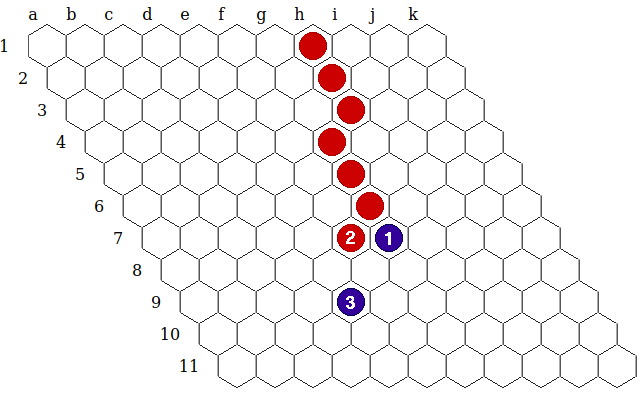
\includegraphics[scale=0.4]{bridge.png}
        \caption{Illustration de la stratégie de bridge}
    \label{fig:bridge}
\end{center}
\end{figure}\\
\subsection{Les heuristiques}
Afin de gagner des parties de Hex il faut penser à créer des joueurs intelligents capables de rivaliser avec succès à l'aide des stratégies gagnantes.\\
Un joueur possède une stratégie gagnante pour un jeu s'il peut s'assurer la victoire quels que soient les coups joués par son adversaire. Par conséquent le but de cette section est d'implémenter des algorithmes décrivant ces stratégies.\\

D'abord, un paradigme important, non seulement pour les jeux compétitifs à deux joueurs (Hex, échecs, Tic Tac Toe...) mais pour la programmation de jeux en général, consiste en des méthodes et des algorithmes évaluant autant de mouvements que possible jusqu'à l'expiration du temps de réflexion.\\

Plusieurs de ces des algorithmes de recherche ont été développés au cours des dernières années, comme \textbf{Minmax (Shannon, 1950), $(\alpha -\beta)$ Pruning (Knuth et Moore, 1975)} qui sera la base de nos joueurs intelligents.\\
\subsubsection{Minmax $(\alpha-\beta)$} \label{minmax}
Le but de cet algorithme est de produire un nombre lié à la possibilité d'une victoire compte tenu de la position actuelle du pion, en essayant de maximiser les gains pour un joueur et les minimiser pour l'autre.\\
Étant donné une position, on suppose que c’est au joueur BLACK de jouer. Dans la position donnée, BLACK a une série de coups qu’il peut effectuer : pour chacun d’eux, il s’interroge sur les répliques éventuelles que peut faire WHITE, qui lui-même analyse pour chacune de ses répliques celles auxquelles peut procéder BLACK, qui à son tour examine à nouveau l’ensemble des coups qu’il peut effectuer suite aux répliques de WHITE, etc.\\

Ce processus de réflexion est généralement associé à \textbf{un arbre} de jeu. Chaque nœud y correspond à une position de jeu  et les branches correspondent aux différents coups que peut faire BLACK ou WHITE à partir de cette position.\\
Cependant le plateau de jeu contient un nombre important de cases, cela fait de très nombreuses combinaisons à comparer, par conséquent il sera impossible d'atteindre des positions terminales. Pour cela, il est nécessaire de mettre en œuvre la stratégie MinMax en utilisant \textbf{une profondeur} d’arbre prédéfinie limitant la recherche; les feuilles de l’arbre ne sont donc pas des positions de fin de jeu, ainsi il n’est pas possible de dire si une feuille correspond à une position gagnante ou à une position perdante. Pour résoudre ce problème, il est ainsi nécessaire de disposer \textbf{d’une fonction d’évaluation (heuristique)}, capable d’estimer le plus précisément possible la qualité d’une position (maximale pour un joueur et minimale pour l'autre ou l'inverse), et qui servira à étiqueter les feuilles de l’arbre par des valeurs numériques. Par la suite on aura deux types de noeuds : un nœud MAX choisit un coup de score maximal parmi ses fils et un nœud MIN choisit un coup de score minimal parmi ses fils.\\
Le nombre de branches que cet algorithme de \textbf{MinMax simple} amène à développer est extrêmement important, soit \textbf{b} la valeur moyenne de ce nombre et \textbf{d} la profondeur ce cette arbre, la complexité de cet algorithme récursif est \textbf{O($b^d$)}, cela implique donc que la fonction d’évaluation doit être appliquée à $b^d$ cases, ainsi la recherche d'un coup va prendra des minutes!! \\

Une amélioration de cet algorithme appelée \textbf{Élagage Alpha-Beta } permet d’éviter de développer des branches inutiles: si la valeur d'un fils $f$ d'un noeud MAX est supérieure à la valeur courante d'un noeud MIN ancêtre, alors les frères de $f$ n'ont pas besoin d'être explorés, ce principe s'appelle \textbf{Coupure Beta}.\\ La figure suivante est un exemple illustrant l'arbre Minmax AlphaBeta: 
\begin{figure}[h]
\begin{center}
    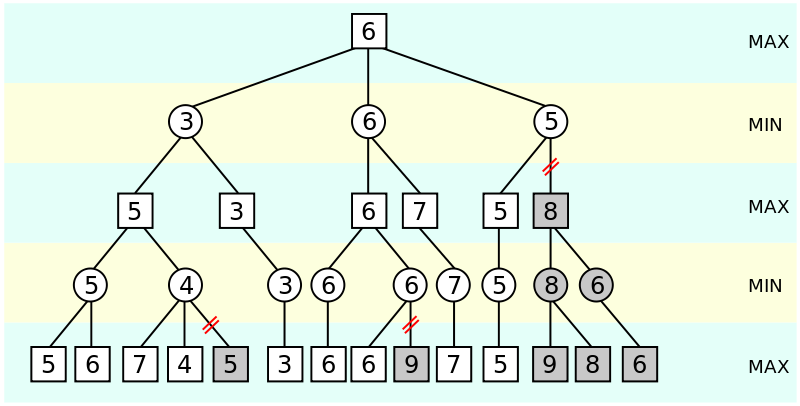
\includegraphics[scale=0.34]{minmax.png}
        \caption{Exemple d'arbe de Minmax AlphaBeta}
    \label{fig:minmax}
\end{center}
\end{figure}\\

Ce processus est décrit par le pseudo-code suivant:\\

\begin{algorithm}
\caption{Élagage Alpha-Beta}
\begin{algorithmic}
\STATE \FuncSty{minmax(position,depth,alpha,beta,bool)}
\STATE
\IF{depth == 0 or game is over}
\RETURN the heuristic of the position\\
\STATE
\ELSIF{player is maximizing (bool==true)}
\STATE maxEval = -inifinie
\FOR{each child of the position} 
\STATE eval = minimax(child, depth - 1, alpha, beta, false)
\STATE maxEval = max(maxEval, eval)
\STATE alpha = max(alpha, eval)
\IF{beta $\leq$ alpha}
\STATE break
\ENDIF
\ENDFOR
\RETURN maxEval\\
\STATE
\ELSE
\STATE minEval = +inifinie
\FOR{each child of the position} 
\STATE eval = minimax(child, depth - 1, alpha, beta, true)
\STATE minEval = min(minEval, eval)
\STATE beta = min(beta, eval)
\IF{beta $\leq$ alpha}
\STATE break
\ENDIF
\ENDFOR
\RETURN minEval
\ENDIF
\end{algorithmic}
\end{algorithm}

Avec \texttt{position} représentant le graphe actuel, et \texttt{child} le graphe fils de \texttt{position} après avoir joué un coup valide dans \texttt{position}.

\subsubsection{Fonction d'évaluation}
Il nous reste maintenant qu'à implémenter \textbf{la fonction d'évaluation (heuristique)}: en intelligence artificielle et optimisation mathématique, une heuristique est une technique conçue pour résoudre un problème plus rapidement lorsque les méthodes classiques sont trop lentes, ou pour trouver une solution approximative lorsque les méthodes classiques ne parviennent pas à trouver une solution exacte.\\
Soit $V$ l'ensemble des cases du plateau, et notant une case par $v$. Supposons que nous connaissions une fonction $f: V \times \{WHITE,BLACK \} \rightarrow R$ qui à chaque position arbitraire $v$ et à chaque joueur $p$ associe $f(v, p)$, représentant la connexité entre les cotés correspondants au plateau du p. Nous supposerons que lorsque les cotés de p sont déjà connectées $f (v, p) = 0$, cette fonction décroît lorsque le joueur est proche de gagner.
Définissons maintenant une fonction d'évaluation $J$ pour Hex comme la différence de connexité entre les deux joueurs:
$$J(v,p)=f(v,p)-f(v,\Bar{p})$$
\begin{itemize}
    \item $J(v,p)$ est positive si le joueur p est le plus proche pour gagner, et négative sinon.
    \item $J(v,p)$ augmente si la connexité entre les bords du plateau de p augmente. 
\end{itemize}
Donc $J(v, p)$ donne une estimation de la valeur stratégique de la position $v$ pour le joueur $p$ qui peut être utilisé dans une recherche minimax. Ensuite, les deux fonctions d'évaluation présentées ci-dessous sont basées sur deux mesures de la connexité relative d'une position dans le plateau du jeu, qui est un concept stratégique très important dans Hex.
\begin{itemize}
    \item \textbf{\texttt{Heeuristic.so}} : La mesure de connexité que nous considérerons dans cette stratégie est :$f_1$.\\ C'est une mesure très simple qui consiste \textbf{à compter le nombre de pièces nécessaires pour connecter les bords} de $p$, il est plus simple de calculer $f_1$ à partir du graphe $G$ associé au plateau de $p$ en calculant \textbf{le chemin le plus court} entre les cotés opposés du plateau avec l'algorithme de \textbf{\texttt{Dijkstra}} (vu au cours de \textbf{la théorie des graphes}) et dont le pseudo-code est le suivant:\\
    \begin{algorithm}
\caption{Algorithme de Dijkstra}
\begin{algorithmic}
\STATE $P = \empty$ //set of vertices included in the shortest path
\STATE $dist[i]= +\infty$ for every vertex i //array of distances from source
\STATE $parent[i]= +\infty$ for every vertex i //array of parents of vertices 
\STATE $dist[source] = 0$
\STATE $parent[source] = -1$
\WHILE{ exists vertex not in P}
\STATE chose a vertex i not in P with minimum distance $dist[i]$
\STATE put i in P 
\FOR{every $v$ neighbour of i \&\& not in P \&\& not marked by the openent \&\& $dist[i] + wight(i,v) \leq dist[v]$} 
\STATE $dist[v] = dist[i] + weight(i,v)$
\STATE $parent[v]=i$
\ENDFOR
\ENDWHILE
\IF{player is BLACK} 
\STATE arrival = Last node
\STATE transforme parent to a path
\RETURN path
\ELSE[player is WHITE]
\STATE arrival = $2\times M+1$ // M is given at the line command (board length)
\STATE transforme parent to a path
\RETURN path
\ENDIF
\end{algorithmic}
\end{algorithm}\\
\textbf{
tel que:
\begin{center}
$weight 
= \begin{cases}
 \text{0  si i et v ont même couleur} \\
 \text{1  si l'une des deux cases est vide } \\
 \text{$+\infty$  si les des deux cases ont des couleurs différentes}\\
 \text{(car l'algorithme ne parcourt pas les pions de l'adversaire) } \\
 \end{cases}$
\\[0.5cm]
\end{center}
}
Le chemin retourné par cet algorithme est donné en paramètre à la fonction \texttt{path\_score} qui est en fait l'implémentation de la métrique $f_1$.\\
Enfin, \texttt{path\_score} est appelée deux fois afin de calculer $f_1(v,p)$ et $f_1(v,\Bar{p})$, ce qui conduit à l'évaluation suivante:
$$J(v,p)=f_1(v,p)-f_1(v,\Bar{p})$$
Par exemple, dans la figure (\ref{fig:heuristique})  suivante l'évaluation pour le joueur WHITE sera $3-7 = -4$
\begin{figure}[h]
\begin{center}
    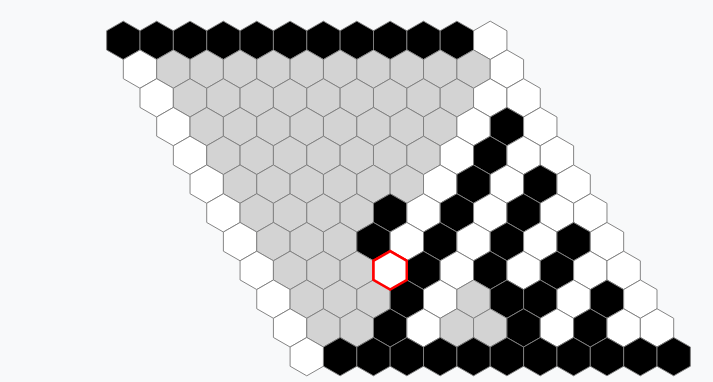
\includegraphics[scale=0.45]{f1.png}
        \caption{Un exemple du plateau où le joueur WHITE est proche de gagner}
    \label{fig:heuristique}
\end{center}
\end{figure}
\item \textbf{\texttt{Heeuristic1.so}}: Le problème avec le comptage du nombre de cellules vides se trouvant dans l'algorithme du plus court chemin, en effet celui ci ne considère pas les chemins alternatifs. Si l'adversaire bloque le chemin le plus court lors de son coup, alors la métrique $f_1$ ne va rien dire sur la connexité du reste du plateau. Nous présentons ici une alternative métrique,$f_2$, qui prend implicitement en compte cette problématique.\\
Considérons le problème de la mesure de la distance $d(u,v)$ entre deux cellules u et v par rapport à un joueur particulier. La métrique $f_1$ utilise la règle suivante : \\
\textbf{
\begin{center}
$d(u,v) 
= \begin{cases}
 weight(u,v)\text{  si u et v sont voisins} \\
 weight(u,v) + d(u',v) \text{  sinon } \\
 \end{cases}$
\\[0.5cm]
\end{center}
}
avec $u'$ est le voisin de $u$ qui a une distance minimale de $v$: $$u'=arg \min_{w \in neighbours(u)} d(w,v) $$
Malheureusement, cette distance conventionnelle est une mauvaise estimation de la valeur d'une position, car au tour suivant, l'adversaire peut placer une pièce sur l'une des cases se trouvant sur le chemin le plus court, sauf si, par hasard, il se produit
être deux ou plusieurs chemins plus courts.\\

On a pensé donc à une meilleure métrique $f_2$ pour Hex dont la valeur augmente pour une position qui a plusieurs chemins de courte longueur entre $u$ et $v$, cette métrique a pour régle: \\

\textbf{
\begin{center}
$d(u,v) 
= \begin{cases}
 weight(u,v)\text{  si u et v sont voisins} \\
 weight(u,v) + d(u',v) \text{  sinon } \\
 \end{cases}$
\\[0.5cm]
\end{center}
}
avec $u''$ est le voisin de $u$ qui a une distance minimale de $v$ après une première suppression de $u'$.\\
Maintenant tout mouvement de blocage potentiel de l'adversaire est pris en compte parce qu'un deuxième alternatif bien connecté, $u''$, est considéré à chaque étape du calcul de la distance. En effet, la métrique fournit des informations de distance sur plusieurs chemins entre u et v.\\

La figure (\ref{fig:heuristique1}) ci-dessous illustre l'idée de la métrique $f_2$, expliquée précédemment, sur une autre représentation du tableau du jeu (où les bords sont représentés par des noeuds extrémistes) \\

\begin{figure}[h]
\begin{center}
    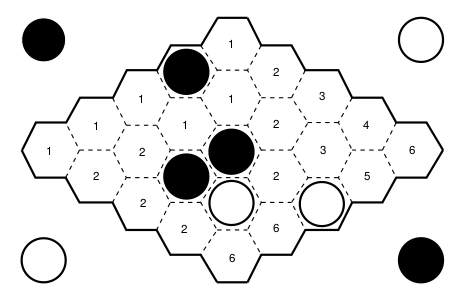
\includegraphics[scale=0.45]{f2.png}
        \caption{Les distances minimales des noeuds par rapport au coté noir en haut à gauche par la métrique $f_2$}
    \label{fig:heuristique1}
\end{center}
\end{figure}


\end{itemize}
\subsubsection{Amélioration} \label{amel}
L'élagage AlphaBeta permet la suppression de grandes branchements dans l’arbre complet. Il en résulte un gain de temps substantiel pour le choix d’un coup à profondeur donnée, en fait si cette profondeur est paire la complexité de notre algorithme sera $O(b*1*b*1..*b)=O(b^{d/2})$ avec b, le nombre moyen des branchements et d la profondeur. On obtiendra le même résultat si la profondeur est impaire.0 En effet, tous les mouvements du premier joueur doivent être étudiés pour trouver le meilleur, mais pour chaque coup parmi ces derniers, seul le meilleur mouvement du deuxième joueur est nécessaire, en fait AlphaBeta garantit qu'aucun autre coup du deuxième joueur ne doit être pris en compte.\\
Cependant, cet algorithme prendra toujours du temps à l'exécution, surtout sur de grands plateaux ($11 \times 11$). \\
Ainsi une première idée était d'introduire le facteur temps : notre heuristique prend un certain temps à calculer, il faut donc estimer ce temps "T", afin que notre Minmax puisse évaluer au plus $n/T$ nœuds. Malheureusement nous n'avons pas réussi à implémenter cette stratégie. Pourtant nous avons pu réduire le temps en évaluant des noeuds prometteurs appartenant \textbf{à l'intersection des plus courts chemin des deux joueurs}
\subsubsection{Choix du meilleur coup} \label{best}
Cette section a pour objectif de rassembler tout ce qui était vu avant en un algorithme donnant le meilleur coup à jouer, nous avons d'abord calculé l'intersection \textbf{I} des plus courts chemin des deux joueurs, ensuite afin que ces stratégies peuvent bloquer l'adversaire nous calculons l'union de \textbf{I} avec les voisins de la dernière case remplie par l'adversaire, noté \textbf{U}. Finalement notre algorithme évalue tous les noeuds appartenant à \textbf{U} en utilisant Minmax et retourne le meilleur coup à jouer. Le pseudo code est le suivant:
    \begin{algorithm}
\caption{Algorithme du choix du meilleur coup}
\begin{algorithmic}
\STATE \texttt{best\_move(board, previous\_move)}
\STATE bestMove = NULL
\FOR{every move in U //U is defined above} 
\IF{current move is better than bestMove} 
\STATE bestMove = current move
\ENDIF
\ENDFOR
\RETURN bestMove
\end{algorithmic}
\end{algorithm}\\
\section{Complexité}
\subsection{Le plateau du jeu}
Le \texttt{TAD graph\_t} et le \texttt{TAD neighbours} fournissent des méthodes qui permettent de manipuler le plateau du jeu, la plupart de ces méthodes sont bonnes en complexité temporelle et spatiale, comme: \texttt{graph\_add\_move}, \texttt{graph\_free}, \texttt{nb\_\_empty}, \texttt{nb\_\_add}, \texttt{nb\_\_free} etc.\\
Cependant la fonction qui permet d'initialiser un graphe (carré ou hexagonale) a une complexité $O(n^2)$ en temps et en espace, avec $n$ le nombre des sommets du graphe, puisqu'elle s'occupe d'allouer les deux matrices \texttt{t} et \texttt{o} de tailles respectives $n^2$ et $2\times n$, et de les parcourir afin de les initialiser.
\subsection{Le serveur}
La complexité du serveur (\emph{ie} de la boucle du jeu) se réduit aux complexités des fonctions \texttt{play} et \texttt{is\_winning}. La complexité de la première varie selon le joueur, \emph{ie} selon la stratégie, alors que la fonction qui détermine si un joueur a remporté une partie, basée sur \textbf{le parcours en profondeur} d'une matrice d'adjacence de taille $n^2$, est en complexité $O(n^2)$.
\subsection{Les clients}
Les fonctions \texttt{get\_player\_name}, \texttt{propose\_opening}, \texttt{accept\_opening}, \texttt{inititalize\_color} et \texttt{finalize}, sont communes pour toutes les interfaces des joueurs \texttt{.c}, elles sont imposées par le sujet, et elles ont une complexité constante en temps et en espace.\\
Il nous reste donc que de parler de la complexité des stratégies implémentées:
\begin{itemize}
    \item \textbf{Le Random \texttt{hero.so}}: Ce joueur tire un nombre aléatoire entre 1 et le nombre de sommets libres N. Ainsi à l’aide du tableau o du graphe, on trouve le ième sommet libre, la complexité de cette stratégie  dans le pire cas est $O(n^2)$
    \item \textbf{\texttt{Bridge.so}}: Ce joueur choisit son coup dans un temps constant, mais il arrive que les cases promotteurs pour lui sont tous remplies, donc il jouera un coup aléatoire de complexité au pire des cas $O(n^2)$.
    \item \textbf{Les heuristiques}: Les stratégies de nos joueurs intelligents sont à base d'un algorithme de Minmax$(\alpha-\beta)$, la complexité de cette algorithme a été bien expliqué dans la section ~\ref{minmax}, elle est égale à $O(b'^{d/2})$ en temps et en espace, avec $b'$ le nombre moyen de branchement, en prenant en considération l'amélioration faite à la section ~\ref{amel}, et $d$ la profondeur de Minmax.\\
    Ensuite la complexité de nos évaluations heuristiques est la complexité de l'algorithme de Dijkstra donc $O(n^2)$.\\
    Finalement la complexité totale en temps de la fonction effectuant le jeu \texttt{play} est $O(b'^{d/2} \times n^2 \times u)$ avec $u = |U|$ (U est l'ensemble décrit à la section \ref{best}), pour $b'$ assez grand cette complexité est réduite à $O(b'^{d/2})$ qui est de même la complexité en espace.

\end{itemize}
\section{Description des tests de validation}
Afin de s'assurer du bon fonctionnement de notre codes, chaque fonction a été dûment vérifiée à l'aide de tests contrôlant leurs résultats pour différents paramètres.

\subsection{Tests sur les stratégies}
Au fur et à mesure de l'avancement du projet nous avons développé différente stratégie afin que notre joueur est de meilleur résultat. Afin de vérifier que ces dernières fonctionnaient correctement nous avons construit une série de tests vérifiant que les résultats de nos fonctions correspondait bien à nos attentes. Afin de réaliser ces tests nous avons utilisé la librairie \texttt{assert} que nous avons importés dans chacun de nos fichiers de test. Pour chacune des stratégies nous réalisons successivement les tests suivant : \\
\begin{itemize}
    \item Nous testons si le graphe est bien initialisé autant dans le cas d'un carré que celui d'un hexagone. \\
    \item Nous nous assurons que la couleur et le nom du joueur utilisant la stratégie est bien définie. \\
    \item Nous vérifions que la stratégie propose un premier coup valable, c'est à dire que ce premier coup appartienne bien au graphe de jeu et qu'il n'ait pas déjà été joué auparavant. \\
    \item Nous faisons jouer le joueur disposant de notre stratégie quelque coups afin de nous assurer du bon fonctionnement de cette dernière. \\
    \item Dans le cas d'une fin de jeu nous vérifions que celle ci est bien détectée.\\
\end{itemize}

Ces tests de base sont valables pour toutes les stratégies, mais pour des stratégies plus poussées comme celle d'\texttt{"heuristic"} des tests supplémentaires sont clairement nécessaires. Cette stratégie mettant en jeu la structure path, nous testons si cette structure est correctement manipulé par nos fonctions, en effet : \\

\begin{itemize}
    \item La stratégie heuristic utilise des paths (chemin) afin d'utiliser ces chemins nous avons eu besoin d'une fonction qui en renvoie un vide prêt à être manipuler nous vérifions donc que la fonction \textit{path\_empty} renvoie bien un chemin vide. \\
    \item Nous avons vérifié que nos fonctions d'ajout et de suppression d'éléments dans un chemin sont bien fonctionnelles dans différents cas. De même pour l'intersection de deux chemins. Pour cela nous avons générés différents chemins et avons opérés différentes opérations sur ceux-ci et vérifier si le résultat obtenu était égal à celui attendu. \\
    \item Ces chemins sont modifiés (rallongé ou raccourci) nous testons donc les fonctions permettant l'ajustement de la mémoire qui leurs est accordé. \\
    
Pour le fonctionnement de la stratégie "heuristic" nous avons besoin de différentes fonctions particulières, comme la fonction minDistance qui renvoie l'indice du sommet non visité d'un graphe correspondant à la distance minimal depuis un sommet donné. Afin de tester ce genre de fonctions nous avons généré plusieurs graphes et avons vérifié que la fonction minDistance renvoyait bien l'indice attendu. Nous avons procédé de la même manière pour les autres fonctions de cette stratégie.

\end{itemize}

\subsection{Tests sur les graphes}
Le jeu peut s'effectuer sur un graphe carré ou hexagonal. Nous avons réalisé des tests permettant de s'assurer que ces graphes étaient initialisés correctement. Pour cela nous avons vérifié pour un sommet du graphe tiré aléatoirement, que ses voisins étaient bien ceux que l'ont devait attendre, selon la géométrie du graphe. Cela nécessite de vérifier une grande quantité de cas, selon que le sommet choisi et au milieu, sur les cotés où sur un coin du graphe.

\section{Discussion}
\subsection{Analyse des résultats obtenus}
Nous avons réussi à implémenter trois stratégies différentes :  \\

\begin{itemize}
    \item Une stratégie qui consiste à choisir aléatoirement un coup parmi les coup disponibles. \\
    \item Une stratégie défensive, qui cherche à empêcher l'adversaire de connecter les bords.  \\
    \item Une stratégie qui reconnaît les coups intéressant, en utilisant l'algorithme d'exploration des arbres : $(\alpha -\beta)$ Minmax.  \\
\end{itemize}

L'objectif de la première stratégie est d'avoir un joueur qui respecte les règles du jeu. Les tests que nous avons effectué ainsi que les résultats des différentes parties, montrent que cet objectif est réussi, car le client \textit{Hero.so}, joue sans produire des erreurs sur le \textit{"Hex score ladder"} .
\newline

L'objectif de la deuxième stratégie, est d'avoir un joueur qui adopte une stratégie défensive. En effet, le client \textit{bridge.so} cherche à profiter du fait qu'il y a toujours un gagnant dans une partie du jeu \textit{Hex}. Par conséquent, s'il empêche son adversaire de gagner, il pourrait être le gagnant de la partie. Cependant, cette stratégie n'est pas basée sur une évaluation intelligente. Ainsi, elle gagne souvent face au joueurs aléatoire, mais elle trouve des difficultés faces aux joueurs intelligents. \\

L'objectif de la troisième stratégie est d'avoir un joueur intelligent, qui est capable de gagner des parties. Les tests que nous avons réalisé nous ont permis de vérifier le bon fonctionnement des deux clients \texttt{heeuristic1.so} et \texttt{heeuristic.so}. De plus, les résultats des parties jouées par ces deux clients, montrent que la stratégie est bien efficace. En effet, la visualisation du déroulement des parties, nous a confirmé que ces deux clients, évaluent les noeuds appartenant à l'intersection des plus courts chemins des deux joueurs, pour choisir leur prochain coup. \\

L'analyse des résultats des différentes parties, montre que le jeu \texttt{Hex}, donne un avantage considérable au joueur qui commence la partie. En effet, la plupart des parties où l'un des clients \texttt{heeuristic.so} ou \texttt{heeuristic1.so} a perdu, étaient celles où il n'a pas joué en premier. D'ailleurs, il gagne souvent face aux mêmes joueurs, quand il joue le premier tour. L'une des solutions qui permettent d'équilibrer le jeu, est la règle du gâteau, qui permet au deuxième joueur de choisir entre intervertir les couleurs, ou accepter le premier coup et jouer à son tour. \\ 


Le classement du \textit{Hex score ladder}, permet de mesurer approximativement l'efficacité de notre stratégie. Cependant, bien que les clients \texttt{heeuristic.so} et \texttt{heeuristic1.so} sont souvent parmi les 5 premiers joueurs dans ce classement, nous ne pouvons pas considérer que notre stratégie est efficace, avant de l'avoir testé contre des êtres humains, ou même des professionnels du jeu \textit{Hex}.

\subsection{Problèmes rencontrés}
\subsubsection{Problèmes liés à l'organisation}
Compte tenu de la situation sanitaire en France, liée à la pandémie du Covid-19, nous étions obligé à travailler ce projet en télétravail. Cette expérience était à la fois difficile et enrichissante. En effet, il était bien plus difficile d’échanger et de communiquer sur le projet et sur nos différents programmes, vu que nous n'avions pas la possibilité de se voir. Par conséquent, nous avons crée un groupe \textit{Facebook} pour pouvoir échanger. Cependant, les échanges par écrit sont souvent lents, c'est pourquoi nous avons décidé de discuter nos différent programmes sur \textit{Discord}. Cette plate-forme, offre la possibilité de partager son écran avec les autres, ce qui est bien pratique pour discuter et expliquer son travail aux autres membres du groupes. Nous avons aussi décidé de mettre un maximum de commentaires à côté de chaque fonction pour permettre à chaque membres du groupe de comprendre le travail des autres.
\newline

Nous avons aussi utilisé la plateforme \textit{Slack}, pour échanger avec notre encadrant Monsieur Frédéric Herbreteau, ainsi que notre responsable de projet Monsieur David Renault.
\newline

Cette situation particulière a mis en valeur l'importance du logiciel de gestion de dépôts \textit{Git}, vu qu'il nous permettait de communiquer nos avancées en temps réel.
%\newline

\subsubsection{Problèmes liés à l'implémentation du jeu}

L'une des difficultés que nous avons rencontré au début de notre travail, était liée au Makefile. En effet, ce qui distingue celui-ci d'un simple programme \textit{Shell}, est la possibilité de ne pas recompiler tous les fichier. Ainsi, il est nécessaire de bien séparer les règles, pour éviter d'exécuter les commandes qui ne sont pas nécessaires. Cette difficulté était une occasion pour revoir notre cours de \textit{PG106 (Programmation impérative 2 et développement logiciel)}, ce qui nous a permis de mieux comprendre la compilation, l'édition des liens ainsi que le Makefile.



\subsection{Limites et améliorations possibles}
%graphe triangulaire
%stratégies
Les discussions entre les différents membres de l'équipe ont montré qu'il est possible d'améliorer notre implémentation.
\newline

En effet, nous avons décidé d'abandonner l'implémentation du graphe triangulaire, afin de nous concentrer sur l'implémentation d'un client qui joue bien. Cependant, nous avons pensé à une méthodes qui pourrait nous aider à trouver la matrice de ce graphe.\\ 


L'idée consiste à remarquer que le graphe triangulaire est constitué par plusieurs hexagonaux. Ainsi, il suffit de considérer un plan, où on introduit une grille, chaque point de cette grille est le centre d'un hexagonal. Ensuite on obtient les sommets du graphe triangulaire par des rotation de 60$^{\circ}$ à partir des centres. \\

Il est possible d'accélérer la stratégie que nous avons implémenté par un algorithme d'apprentissage. Cependant, la quantité de l'information à apprendre est gigantesque, d'où l'importance des neurones, ces derniers sont des unités de calcul qui contiennent un certain nombre d'entrées et une sortie ce qui permet de s'approcher du comportement du cerveau. Ainsi, il est nécessaire d'utiliser une bibliothèque comme FANN (\textit{Fast Artificial Neural Network }). En effet, cette bibliothèque peut être utilisée par plusieurs langages de programmation (C, C++, PHP,Python ...). De plus, elle utilise le principe de l'approximation fonctionnelle, ce qui signifie qu'elle apprend une fonction par le biais de plusieurs exemples de cette fonction. Ainsi, on peut espérer obtenir des résultats correcte, quand on lui donnera une nouvelle entrée. \\

Nous avons commencé à nous renseigner sur la bibliothèque FANN, mais nous avons fini par abandonner cette méthode par manque de temps. En effet, cette méthode n'intervient qu'après avoir implémenté une stratégie gagnante efficace. Nous avons donc préféré améliorer notre code ainsi que notre rapport. 


    


\section{Conclusion}
Ce projet a permis à l'ensemble des membres du groupe de s'épanouir et d'acquérir de nouvelles compétences. C'était aussi l'occasion de mieux comprendre plusieurs parties de notre cours comme les graphes, la compilation, l'édition des liens et le Makefile. 
\newline

De plus, il nous a permis d'apprendre à gérer le travail en groupe, même dans cette situation particulière où nous devons travailler à distance  compte tenu des mesures de confinement, liées à la pandémie du Covid19. Les différentes discussions entre les membre de l'équipe furent constructives puisque composées de quatre pointe de vues différents.
\newline

L'outil \textit{Hex score ladder}, qui permet de classer les différents joueurs et de visualiser le déroulement de chaque partie, a ajouté une touche d'amusement et de compétitivité, ce qui nous a motivé à faire  évoluer notre code.
\newline

Nous tenons à remercier notre encadrant  Monsieur Frédéric Herbreteau, ainsi que notre responsable de projet Monsieur David Renault pour toute l'aide qu'ils nous ont apporté.


\section{Références}

https ://www.labri.fr/perso/renault/working/teaching/projets/
\\
\indent https ://thor.enseirb-matmeca.fr/
\\
\indent https://www.labri.fr/perso/renault/working/teaching/projets/ladder/ladder.html
\\
\indent https://www.gnu.org/software/gsl/
\\
\indent http://tldp.org/HOWTO/Program-Library-HOWTO/dl-libraries.html

\end{document}
